% Minimal TikZ standalone example
\documentclass[tikz, border=1mm]{standalone}

\usepackage{amsmath,amssymb}
\usepackage{tikz}

\usetikzlibrary{calc}
\usetikzlibrary{angles,quotes}

\begin{document}
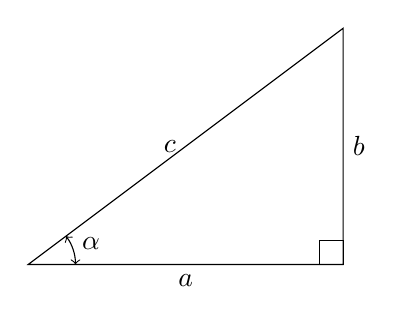
\begin{tikzpicture}
	\coordinate (A) at (0,0);
	\coordinate (B) at (4,0);
	\coordinate (C) at (4,3);

	% Triangle
	\draw (A) -- (B) -- (C) -- cycle;

	% Right angle mark
	\draw (B) rectangle +(-0.3,0.3);

	% Vertex labels
	%\node[below left]  at (A) {$A$};
	%\node[below right] at (B) {$B$};
	%\node[above left]  at (C) {$C$};

	% Side labels (a opposite A, etc.)
	\node[below] at ($(A)!0.5!(B)$) {$a$};
	\node[left]  at ($(A)!0.5!(C)$) {$c$};
	\node[right] at ($(B)!0.5!(C)$) {$b$};

	% Angle labels
	\pic["$\alpha$", draw, <->, angle eccentricity=1.4, angle radius=0.6cm]
		{angle = B--A--C};
\end{tikzpicture}
\end{document}
